\section{Differential Forms in Geometric Calculus}
\subsection{Inner Products of Subspaces}\label{sect5_6_1}
Start by considering products of the form where $A_{r}$ and $B_{r}$ are $r$-grade blades
\be
 A^{\R}_{r}\cdot B_{r} = \paren{a_{1}\W\dots\W a_{r}}^{\R}\cdot\paren{b_{1}\W\dots\W b_{r}}
\ee
Both $A_{r}$ and $B_{r}$ define $r$-dimensional subspaces of the vector space via the equations $x\W A_{r} = 0$ and $x\W B_{r} = 0$.  
We show that if $A_{r}$ and $B_{r}$ do not 
define the same subspace then $A^{\R}_{r}\cdot B_{r} = 0$. Assume that they do not define the same subspaces, but
that the intersection of the subspaces has dimension $s<r$ so that one can have an orthogonal basis for $A_{r}$ of
$\Set{e_{1},\dots,e_{s},e_{s+1},\dots,e_{r}}$ and an orthogonal basis for $B_{r}$ of $\Set{e_{1},\dots,e_{s},e'_{s+1},\dots,e'_{r}}$. 
Then the geometric product of $A^{\R}_{r}$ and $B_{r}$ is
\begin{align}
 A^{\R}_{r}B_{r} &= \alpha e_{r}\dots e_{s+1}e_{s}\dots e_{1}\beta e_{1}\dots e_{s}e'_{s+1}\dots e'_{r} \nonumber \\
            &= \paren{\alpha\beta e_{1}^{2}\dots e_{s}^{2}}e_{s+1}\dots e_{1}e'_{s+1}\dots e'_{r}
\end{align}
where the quantity in parenthesis is a scalar and the other factors a blade of grade $2\paren{r-s}$. Thus 
\be\label{eq5_145}
	A^{\R}_{r}\cdot B_{r} = \braket{A^{\R}_{r}B_{r}} = 0.
\ee
If $A_{r}$ and $B_{r}$ define the same $r$-dimensional subspace let $\Set{e_{1},\dots, e_{r}}$ be an orthogonal basis for the subspace and
expand $A_{r}$ and $B_{r}$ in terms of the orthogonal basis vectors and reciprocal orthogonal basis vectors respectively -
\be\label{eq5_141}
	a_{i} = \paren{a_{i}\cdot e^{j}}e_{j}
\ee
and 
\be\label{eq5_142}
	b_{i} = \paren{b_{i}\cdot e_{j}}e^{j}
\ee
Let the matrices of the coefficients in equations~\ref{eq5_141} and \ref{eq5_142} be denoted by $\Mat{a_{i}\cdot e^{j}}$ and 
$\Mat{b_{i}\cdot e_{j}}$.  Then we can expand $A_{r}$ and $B_{r}$ as
\be
	A_{r} = \det\paren{\Mat{a_{i}\cdot e^{j}}}e_{1}\dots e_{r}
\ee
and
\be
	B_{r} = \det\paren{\Mat{b_{i}\cdot e_{j}}}e^{1}\dots e^{r}
\ee
and (since the determinant of a matrix and determinant of the transpose of matrix are equal)
\begin{align}
A^{\R}_{r}\cdot B_{r} &= \det\paren{\Mat{a_{i}\cdot e^{j}}}\det\paren{\Mat{b_{i}\cdot e_{j}}}\braket{e_{r}\dots e_{1}e^{1}\dots e^{r}} \nonumber \\
                      &= \det\paren{\Mat{a_{i}\cdot e^{j}}}\det\paren{\Mat{b_{i}\cdot e_{j}}} \nonumber \\
                      &= \det\paren{\Mat{a_{i}\cdot e^{j}}}\det\paren{\Mat{b_{i}\cdot e_{j}}^{T}} \nonumber \\
                      &= \det\paren{\Mat{a_{i}\cdot e^{j}}}\det\paren{\Mat{b_{j}\cdot e_{i}}} \nonumber \\
                      &= \det\paren{\Mat{\paren{a_{i}\cdot e^{k}}\paren{b_{j}\cdot e_{k}}}}
\end{align}
But 
\begin{align}
 a_{i}\cdot b_{j} &= \paren{a_{i}\cdot e^{k}}e_{k}\cdot\paren{b_{j}\cdot e_{l}}e^{l} \nonumber \\
                  &= \paren{a_{i}\cdot e^{k}}\paren{b_{j}\cdot e_{l}}\delta^{l}_{k} \nonumber \\
                  &= \paren{a_{i}\cdot e^{k}}\paren{b_{j}\cdot e_{k}}
\end{align}
So that
\be
A^{\R}_{r}\cdot B_{r} = \det\paren{\Mat{a_{i}\cdot b_{j}}}.
\ee
From our derivations we see that if $A_{r}$ is a general $r$-grade multivector (not a blade) we can always find a $r$-grade blade such that
\be
	A^{\R}_{r}\cdot\paren{b_{1}\W\dots\W b_{r}} = \paren{a_{1}\W\dots\W a_{r}}^{\R}\cdot\paren{b_{1}\W\dots\W b_{r}}.
\ee
Now consider the relation between the basis $\Set{a_{1},\dots, a_{n}}$ and the reciprocal basis $\Set{a^{1},\dots, a^{n}}$ for an $n$-dimensional vector space where 
in equation~\ref{eq5_149} $r \le n$ and $1 \le i_{l},j_{m} \le n$
\be\label{eq5_149}
	\paren{a_{i_{1}}\W\dots\W a_{i_{r}}}^{\R}\cdot\paren{a^{j_{1}}\W\dots\W a^{j_{r}}} = \det\paren{\Mat{a_{i_{l}}\cdot a^{j_{m}}}} = \det\paren{\Mat{\delta_{i_{l}}^{j_{m}}}}
\ee
where $i_{1}<i_{2}<\dots<i_{r}$ and  $j_{1}<j_{2}<\dots<j_{r}$.  Equation~\ref{eq5_149} is zero unless $i_{l}=j_{l}$ for all $1\le l \le r$ so that
\be
    \paren{a_{i_{1}}\W\dots\W a_{i_{r}}}^{\R}\cdot\paren{a^{j_{1}}\W\dots\W a^{j_{r}}} = \delta_{i_{1}}^{j_{1}}\delta_{i_{2}}^{j_{2}}\dots\delta_{i_{r}}^{j_{r}}.
\ee
since if the index ordering condition is satisfied for the $i_{l}$'s and the $j_{m}$'s and there is an index, $l$, such that $i_{l} \ne j_{l}$ then the two blades do not
define the same subspace and the inner product is zero.  The square of a blade is given by
\begin{align}
	\paren{a_{1}\W\dots\W a_{r}}^{2} &= \paren{a_{1}\W\dots\W a_{r}}\cdot\paren{a_{1}\W\dots\W a_{r}} \\
	                               &= \paren{-1}^{\frac{r(r-1)}{2}}\paren{a_{1}\W\dots\W a_{r}}^{\R}\cdot\paren{a_{1}\W\dots\W a_{r}} \\
	                               &= \paren{-1}^{\frac{r(r-1)}{2}}\f{\det}{\Mat{a_{i}\cdot a_{j}}} \label{eq5_158}\\
	                               &= \paren{-1}^{\frac{r(r-1)}{2}}a_{1}^{2}\dots a_{r}^{2} \mbox{ if the $a_{i}$'s are orthogonal}.
\end{align}

\subsection{Alternating Forms}
If $V$ is a vector space then an $r$-rank tensor is a multilinear map
\be
	\f{T_{r}}{v_{1},\dots,v_{r}}:\bigotimes\limits_{i=1}^{r}V\rightarrow\mathcal{R}
\ee
where ($\otimes$ is the cartesian product of vector spaces)
\be
	\bigotimes\limits_{i=1}^{r}V = \underbrace{V\otimes\dots\otimes V}_{\mbox{$r$ times}}
\ee
so that if $v_{i}\in V$ the tuple $\paren{v_{1},\dots,v_{r}}\in \bigotimes\limits_{i=1}^{r}V$.

The sum of two $r$-rank tensors is the $r$-rank tensor defined by
\be
	\f{\paren{A_{r}+B_{r}}}{v_{1},\dots,v_{r}} \equiv \f{A_{r}}{v_{1},\dots,v_{r}}+\f{B_{r}}{v_{1},\dots,v_{r}}.
\ee
The tensor product of rank $r$ and $s$ tensors is a rank $r+s$ tensor defined by
\be
	\f{\paren{A_{r}\otimes B_{s}}}{v_{1},\dots,v_{r+s}} \equiv \f{A_{r}}{v_{1},\dots,v_{r}}\f{B_{s}}{v_{r+1},\dots,v_{r+s}}.
\ee
An $r$-form (when we say something is a form from now on we mean alternating form) is an $r$-rank tensor with the property (no summation in this case)
\be
\f{\alpha_{r}}{v_{1},\dots,v_{r}} = \epsilon^{i_{1}\dots i_{r}}_{1\dots r}\f{\alpha_{r}}{v_{i_{1}},\dots,v_{i_{r}}}
\ee
where $\epsilon^{i_{1}\dots i_{r}}_{1\dots r}$ is the mixed rank permutation symbol.  We can always construct an $r$-form from an $r$-rank tensor via 
\be
	\f{\alpha_{r}}{v_{1},\dots,v_{r}} = \f{\epsilon}{A_{r}} \equiv \sum_{i_{1},\dots,i_{r}}\epsilon_{i_{1}\dots i_{r}}^{1\dots r}\f{A_{r}}{v_{i_{1}},\dots,v_{i_{r}}}
\ee
In the geometric algebra a simple representation of an alternating $r$-form is
\be
	\f{\alpha_{r}}{v_{1},\dots,v_{r}} = A^{\R}_{r}\cdot\paren{v_{1}\W\dots\W v_{r}}
\ee
where $A_{r}$ is a grade-$r$ multivector.  Since the grade of $A_{r}$ and the grade of $\paren{v_{1}\W\dots\W v_{r}}$ are the same the 
inner product results in a scalar and also since $\paren{v_{1}\W\dots\W v_{r}}$ is a blade it alternates sign upon exchange of adjacent
vectors.

The basic operations of the ``Algebra of Forms'' inherit the sum and cartesian product operations from tensor since they are tensors.  However, 
in order to construct an algebra of forms we need a product of two forms that results in a form.  The tensor product of two alternating forms is
not an alternating form, but since we know how to convert a tensor to a form we define the exterior product of an $r$-form and $s$-form to be 
the $r+s$ form
\be\label{eq5_158}
	\alpha_{r}\Wbld \beta_{s} \equiv \f{\epsilon}{\alpha_{r}\otimes\beta_{s}}
\ee
as an example
\be
	\f{\alpha_{1}}{v_{1}}\Wbld\f{\beta_{1}}{v_{2}} = \f{\alpha_{1}}{v_{1}}\f{\beta_{1}}{v_{2}}-\f{\alpha_{1}}{v_{2}}\f{\beta_{1}}{v_{1}}
\ee
so that
\be
\f{\alpha_{r}}{v_{1},\dots,v_{r}}\Wbld\f{\beta_{s}}{v_{r+1},\dots,v_{r+s}} = \paren{A_{r}\W B_{s}}^{\R}\cdot\paren{v_{1}\W\dots\W v_{r+s}}
\ee
and
\be
	\alpha_{r}\Wbld\beta_{s} = \paren{-1}^{rs}\beta_{s}\Wbld\alpha_{r}
\ee
The interior product of an $r$ and $s$-form is defined by ($r > s$) an $r-s$ form (note that we are distinguishing the inner, $\cdotbld$, and
exterior, $\Wbld$, products for forms from the geometric algebra products by using boldface symbols)
\be
\beta_{s}\cdotbld\alpha_{r} \equiv \paren{B_{s}\cdot A_{r}}^{\R}\cdot\paren{v_{s+1}\W\dots\W v_{r}}
\ee
A $r$-form is simple if $A_{r}$ is a blade ($A_{r} = a_{1}\W\dots\W a_{r}$).

\subsection{Dual of a Vector Space}
Let $V$ be a $n$-dimensional vector space.  The set of all linear maps $f:V\rightarrow \mathcal{R}$ is denoted $V^{*}$ and is a vector space called the
dual space of $V$. $V^{*}$ is a $n$-dimensional vector space since for $f,g:V\rightarrow \mathcal{R}$, $x \in V$, $\alpha \in \mathcal{R}$ and we define
\begin{align}
	\f{\paren{f+g}}{x} \equiv \f{f}{x} +\f{g}{x} \\
	\f{\paren{\alpha f}}{x} \equiv \alpha\f{f}{x} \\
	\f{0}{x} \equiv 0
\end{align}
Then by the linearity of $\f{f}{x}$ and $\f{g}{x}$, $\f{\paren{f+g}}{x}$, $\f{\alpha f}{x}$, and $\f{0}{x}$ are also linear functions of $x$ and $V^{*}$ is
a vector space.

Let $\mathbf{e}_{i}$ be a basis for $V$ and define $\sigma^{i} \in V^{*}$ by
\be
	\f{\sigma^{i}}{\mathbf{e}_{j}} = \delta_{j}^{i}
\ee
so that if $x = x^{i}\mathbf{e}_{i} \in V$ then
\be
	\f{\sigma^{i}}{x} =  \f{\sigma^{i}}{x^{j}\mathbf{e}_{j}} = x^{i} 
\ee
so that for any $f \in V^{*}$
\be
	\f{f}{x} = \f{f}{x^{i}\mathbf{e}_{i}} = x^{i}\f{f}{\mathbf{e}_{i}}
\ee
Now assume that
\begin{align}
	0 &= a_{i}\f{\sigma^{i}}{\mathbf{e}_{j}} \\
	  &= a_{i}\delta_{j}^{i} \\
	  &= a_{j} 
\end{align}
so the $\sigma^{i}$ are linearly independent. Now assume $f \in V^{*}$.  Then
\begin{align}
	\f{f}{x} &= \f{f}{x^{i}\mathbf{e}_{i}} \\
	         &= x^{i}\f{f}{\mathbf{e}_{i}} \\
	         &= \f{f}{\mathbf{e}_{i}}\f{\sigma^{i}}{x} \\
	         &= \f{\paren{\f{f}{\mathbf{e}_{i}}\sigma^{i}}}{x}
\end{align}
Thus
\be
	f = \f{f}{\mathbf{e}_{i}}\sigma^{i}
\ee
and the $\sigma^{i}$ form a basis for $V^{*}$.  If the $\mathbf{e}_{i}$ form an 
orthonormal basis for $V$ (remember that orthonomal implies orthogonal and orthogonal
implies that a dot product is defined since the dot product is used to define orthogonal) then
\be
	\f{\sigma^{i}}{x} = \mathbf{e}_{i}\cdot x.
\ee
Since for 1-forms, $\alpha:V\rightarrow\mathcal{R}$, we have $\alpha\in V^{*}$.  The most
general 1-form can be written
\be
	\f{\alpha}{v} = \alpha_{i}\f{\sigma^{i}}{v}.
\ee
If $\alpha$ is a 2-form, $\f{\alpha}{v_{1},v_{2}}$, the bases are $\sigma^{i}\Wbld\sigma^{j}$, and
the most general 2-form is written as
\be
	\f{\alpha}{v_{1},v_{2}} = \sum_{i<j}\alpha_{ij}\f{\sigma^{i}}{v_{1}}\Wbld\f{\sigma^{j}}{v_{2}}	
\ee
since $\sigma^{i}\Wbld\sigma^{i}=0$ and $\sigma^{i}\Wbld\sigma^{j}=-\sigma^{i}\Wbld\sigma^{j}$ from
the definition in equation~\ref{eq5_158}.

\subsection{Standard Definition of a Manifold}
Let $\mathcal{M}^{n}$ be any set\footnote{This section is based upon sections 1.2 and 2.1 in 
``The Geometry of Physics, An Introduction (Second Edition),'' by T. Frankel} that has 
a covering of subsets, $\mathcal{M}^{n} = U\cup V\cup\dots$ such that
\begin{enumerate}
	\item For each subset $U$ there is a one to one mapping $\phi_{U}:U\rightarrow\mathcal{R}^{n}$ where $\f{\phi_{U}}{U}$ is an 
	open subset of $\mathcal{R}^{n}$.
	\item Each $\f{\phi_{U}}{U\cap V}$ is an open subset of $\mathcal{R}^{n}$.
	\item The overlap maps
		\be
			f_{UV}= \phi_{V}\circ\phi_{U}^{-1}: \f{\phi_{U}}{U\cap V}\rightarrow\mathcal{R}^{n}
		\ee
	or equivalently the compound maps
		\be
			\f{\phi_{U}}{U\cap V}\stackrel{\phi_{U}^{-1}}{\longrightarrow}\mathcal{M}^{n}\stackrel{\phi_{V}}{\longrightarrow}\mathcal{R}^{n}
		\ee
	are differentiable.
	\item Take a maximal atlas of coordinate patches $\Set{(U,\phi_{U}),(V,\phi_{V}),\dots}$ and define a topology for $\mathcal{M}^{n}$ by defining
	that a subset $W\subset \mathcal{M}^{n}$ is open if for any $p \in W$ there is a $(U,\phi_{U})$ such that $p\in U\subset W$.
\end{enumerate}
If the resulting topology for $\mathcal{M}^{n}$ is Hausdorff and has a countable base we say $\mathcal{M}^{n}$ is an $n$-dimensional differentiable manifold 
(look it up since I don't know what it means\footnote{G. Simmons,{\em Topology and Modern Analysis}, McGraw-Hill,1963}).

Figure~\ref{fig5_3} (page 94) shows the relationships between the Manifold and the coordinate patch mappings.

\begin{figure}[htbp]
\begin{center}
\scalebox{0.75}{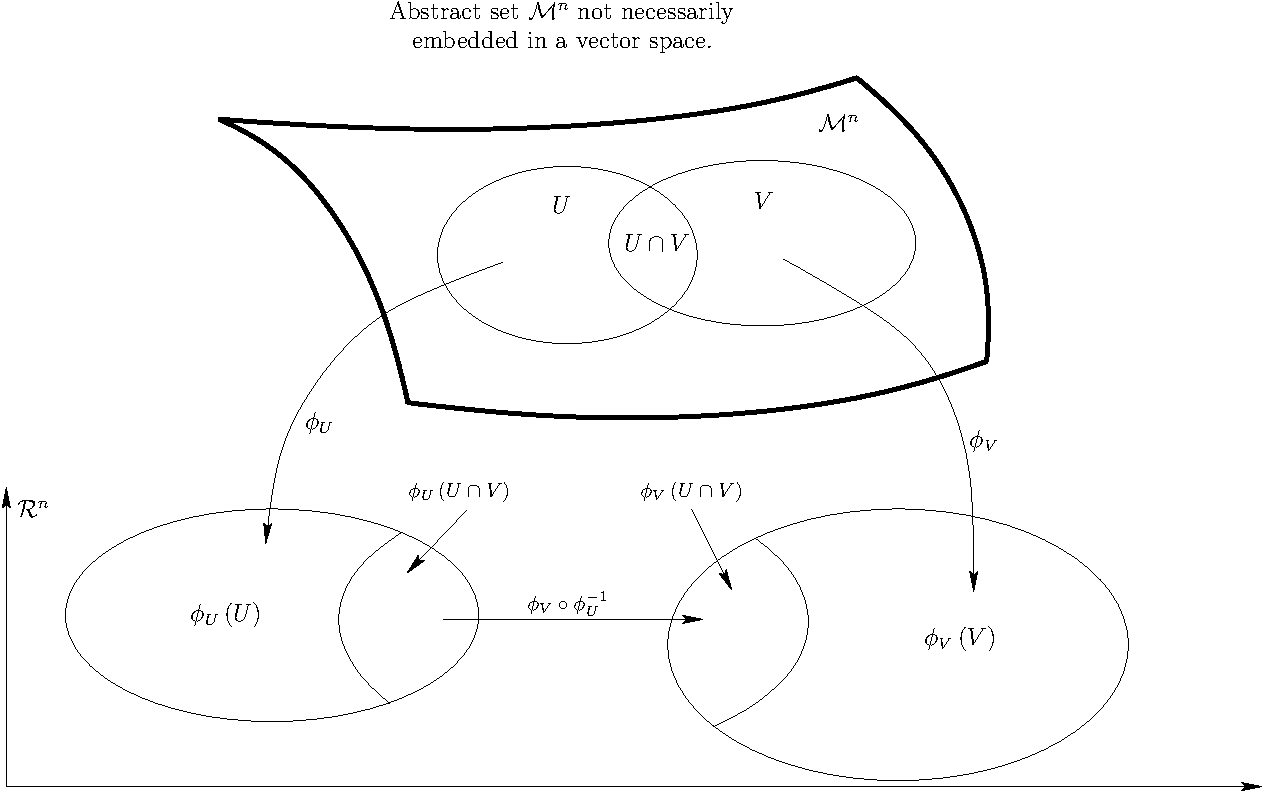
\includegraphics{manifolddef_crop.pdf}}
\caption{Fundamental Manifold Mappings.}\label{fig5_3}
\end{center}
\end{figure}

If $f:\mathcal{M}^{n}\rightarrow\mathcal{R}$ is a real valued function on the manifold $\mathcal{M}^{n}$ it is differentiable if $f_{U} = f\circ\phi_{U}^{-1}$
is differentiable with respect to the coordinates $\Set{x^{1}_{U},\dots, x^{n}_{U}}$ for any coordinate patch $(U,\phi_{U})$.  The real scalars 
$\Set{x^{1}_{U},\dots, x^{n}_{U}}$
(denoted by the tuple $x=\paren{x^{1}_{U},\dots,x^{n}_{U}}$) form a coordinate system for $\f{\phi_{U}}{U} \subset \mathcal{R}^{n}$.  In the future we shall simply
say that $f$ is differentiable if $f_{U}$ is differentiable.  Likewise we will shall usually omit the process of replacing $f$ by its composition 
$f\circ\phi_{U}^{-1}$, thinking of $f$ as directly expressible as a function $\f{f}{x} = \f{f}{x^{1}_{U},\dots,x^{n}_{U}}$ of any local coordinates.

Now let $p \in U\cap V \subset \mathcal{M}^{n}$ and 
\be
	x_{U} = \paren{x_{U}^{1},\dots,x_{U}^{n}} = \f{\phi_{U}}{p}\mbox{ and }x_{V} = \paren{x_{V}^{1},\dots,x_{V}^{n}} = \f{\phi_{V}}{p}. \nonumber
\ee
Then
\be
	x_{U} = \f{\phi_{U}\circ\phi_{V}^{-1}}{x_{V}}=\f{x_{U}}{x_{V}}\mbox{ and } x_{V} = \f{\phi_{V}\circ\phi_{U}^{-1}}{x_{U}}=\f{x_{V}}{x_{U}}. \nonumber
\ee
Let $X_{U} = \paren{X_{U}^{1},\dots,X_{U}^{n}}$ and consider the linear approximation to $\f{\phi_{V}\circ\phi_{U}^{-1}}{x_{U}+hX_{U}}$ where $h$ is a 
small number. Then in the linear approximation
\be
	\f{\phi_{V}\circ\phi_{U}^{-1}}{x_{U}+hX_{U}} = \f{x_{V}}{x_{U}}+h\mat{\pdiff{x_{V}^{i}}{x_{U}^{j}}}X_{U}^{T} = x_{V}+hX_{V}
\ee
so that
\be\label{eq5_161}
	X_{V}^{i} = \pdiff{x_{V}^{i}}{x_{U}^{j}}X_{U}^{j}
\ee
where $\mat{\pdiff{x_{V}^{i}}{x_{U}^{j}}}$ is the Jacobian matrix of the coordinate transformation from one coordinate patch to another and $X_{U}^{T}$ is the 
transpose (colume vector) of the tuple $X_{U}$ (row vector).  
\subsection{Tangent Space}
Now consider the case of a vector manifold in Euclidian space.  The definition of the tangent vector generalizes the concept of the directional derivative
in $\mathcal{R}^{n}$. if $X_{p}$ is a vector at point $p \in \mathcal{R}^{n}$ and $f:\mathcal{R}^{n}\rightarrow\mathcal{R}$ is a $C^{\infty}$ function in
the neighborhood of $p$ then define
\be
	\f{X_{p}}{f} \equiv X_{p}\cdot\Eval{\nabla f}{p}.
\ee
If $f$ and $g$ are $C^{\infty}$ and $\alpha,\beta \in \mathcal{R}$ we have (from the properties of $\cdot$ and $\nabla$)
\begin{align}
	\f{X_{p}}{\alpha f+\beta g} &= \alpha\f{X_{p}}{f} + \beta \f{X_{p}}{g} \\
	\f{X_{p}}{fg} &= \f{f}{p}\f{X_{p}}{g} + \f{g}{p}\f{X_{p}}{f}
\end{align}
Let $\f{C^{\infty}}{p}$ denote the set of real functions that are $C^{\infty}$ on some neighborhood of $p \in \mathcal{M}^{n}$. The generalization 
of the tangent vector to an abstract manifold at a point $p \in \mathcal{M}^{n}$ is defined as a real valued function $X_{p}: \f{C^{\infty}}{p}\rightarrow\mathcal{R}$
such that ($f,g \in \f{C^{\infty}}{p}$ and $\alpha \in \mathcal{R}$)
\begin{align} 
	\f{X_{p}}{f+g} &= \f{X_{p}}{f}+\f{X_{p}}{g} \label{eq5_187}\\
	\f{X_{p}}{\alpha f} &= \alpha\f{X_{p}}{f} \label{eq5_188}\\
	\f{X_{p}}{fg} &= \f{f}{p}\f{X_{p}}{g}+\f{g}{p}\f{X_{p}}{f}.\label{eq5_189}
\end{align}
A tangent vector is often called a derivation on $\f{C^{\infty}}{p}$.  For a given coordinate patch $\paren{U,\phi_{U}}$ we define the tangent space basis
vectors $\paren{\pdiff{}{x^{i}_{U}}}_{p}$ by 
\be\label{eq5_190}
	\Pval{\pdiff{}{x^{i}_{U}}}{p}f \equiv \Eval{\pdiff{\paren{f\circ\phi^{-1}_{U}}}{x^{i}_{U}}}{\f{\phi_{U}}{p}}.
\ee
Since they are partial derivatives the $\Pval{\pdiff{}{x^{i}_{U}}}{p}$ trivially satisfy equations~\ref{eq5_187}, \ref{eq5_188}, and \ref{eq5_189}.  The
general tangent vector is then given by the scalar linear differential operator
\be
	X_{p} = X^{i}_{U}\Pval{\pdiff{}{x^{i}_{U}}}{p}
\ee
Thus we require for $X_{p}$
\be
	\f{X_{p}}{f} = X^{i}_{U}\Pval{\pdiff{}{x^{i}_{U}}}{p}f = X^{j}_{V}\Pval{\pdiff{}{x^{j}_{V}}}{p}f
\ee
for all $p \in U\cap V$.  Thus
\begin{align}
	X^{i}_{U}\Pval{\pdiff{}{x^{i}_{U}}}{p}f &= X^{j}_{V}\Pval{\pdiff{}{x^{j}_{V}}}{p}f \\
	X^{i}_{U}\Pval{\pdiff{x^{k}_{V}}{x^{i}_{U}}}{p}\Pval{\pdiff{}{x^{k}_{V}}}{p}f &= X^{j}_{V}\Pval{\pdiff{}{x^{j}_{V}}}{p}f
\end{align}
and
\be\label{eq5_195}
	X^{j}_{V} = X^{i}_{U}\Pval{\pdiff{x^{j}_{V}}{x^{i}_{U}}}{p}
\ee
is the transformation law for the components, $X^{i}_{U}$, of the tangent vectors.

We have established an isomorphism between the tuple $\paren{X^{1}_{U},\dots,X^{n}_{U}}$ that transforms as in equation~\ref{eq5_161} and the scalar
linear operator $X_{p}$ so that
\be
	\paren{X^{1}_{U},\dots,X^{n}_{U}} \Leftrightarrow X^{i}_{U}\pdiff{}{x^{i}_{u}}
\ee
since 
\be
	X_{U}^{i}\pdiff{f}{x_{U}^{i}} = X_{V}^{j}\pdiff{f}{x_{V}^{i}},\:\:\forall\:f:\mathcal{M}^{n}\rightarrow\mathcal{R}
\ee
implies equation~\ref{eq5_161}.
A vector field on a manifold is then a tangent vector with coefficients, $\f{X^{i}}{p}$ that are functions of the position $p$ on the manifold 
so that ($x_{U} = \paren{x^{1}_{U},\dots,x^{n}_{U}}$) 
\be\label{eq5_205}
	\f{X}{p} = \f{X_{U}}{x_{U}} = \f{X^{i}_{U}}{x_{U}}\Pval{\pdiff{}{x^{i}_{U}}}{p} = \f{X^{i}_{U}}{x^{1}_{U},\dots,x^{n}_{U}}\Pval{\pdiff{}{x^{i}_{U}}}{p}
\ee
and the coefficients $\f{X^{i}_{U}}{x_{U}}$ transform under a change of basis according to equation~\ref{eq5_195}.

\subsection{Differential Forms and the Dual Space}

If $f:\mathcal{M}^{n}\rightarrow\mathcal{R}$ we define the differential of $f$ at $p\in\mathcal{M}^{n}$, $df:\mathcal{M}^{n}_{p}\rightarrow\mathcal{R}$
where $X_{p}\in\mathcal{M}^{n}_{p}$ as the linear functional
\be
	\f{df}{X} \equiv \f{X_{p}}{f}
\ee
so that in general case of $X$ being a vector field (we are supressing the the patch index $U$)
\be
	\f{df}{\f{X}{p}} = \f{df}{\f{X^{i}}{p}\Pval{\pdiff{}{x^{i}}}{p}} = \f{X^{i}}{p}\Eval{\pdiff{f}{x^{i}}}{p}.
\ee
If $\f{f}{p}=\f{x^{i}}{p}$ are the coordinate functions we have
\be
	\f{dx^{i}}{\Pval{\pdiff{}{x^{j}}}{p}} = \Eval{\pdiff{x^{i}}{x^{j}}}{p} = \delta^{i}_{j}
\ee
and
\be
	\f{dx^{i}}{\f{X}{p}} = \f{dx^{i}}{\f{X^{j}}{p}\Pval{\pdiff{}{x^{j}}}{p}} = \f{X^{j}}{p}\f{dx^{i}}{\Pval{\pdiff{}{x^{j}}}{p}} = \f{X^{i}}{p}.
\ee

Consider what this means in a vector manifold where the point $p$ on the manifold is a vector in the embedding vector space.  Then the coordinate
functions $\f{x^{i}}{p}$ can be inverted and the manifold defined by $\f{p}{x^{1},\dots,x^{n}}$.  Knowing the tuple $\paren{x^{1},\dots,x^{n}}$ lets
one calculate the vector $p$ on the manifold.  Then the basis tangent vectors are $e_{i} = \pdiff{p}{x^{i}}$ and the general tangent vector is
$X_{p}= X^{i}e_{i} = X^{i}\pdiff{p}{x^{i}}$.  Now let $\f{f}{p}=\f{f}{x^{1},\dots,x^{n}}:\mathcal{R}^{n}\rightarrow\mathcal{R}$ be a function from
the manifold to the scalars and denote the directional derivative of $f$ as
\be
	\f{df}{X_{p}} = X\cdot\eval{\nabla f}{p} = X^{i}\eval{\pdiff{f}{x^{i}}}{p}
\ee
which is the same as equation~\ref{eq5_205} and the justification for defining the tangent vectors as the linear scalar differential operator 
$X_{p} = X^{i}\eval{\pdiff{}{x^{i}}}{p}$.
What is called the differential operator in the language of differential forms becomes the directional derivative on a vector manifold.

The $dx^{i}$ form a basis for the dual space $\mathcal{M}^{n*}_{p}$.  The most general element of $\mathcal{M}^{n*}_{p}$ can then be written as
\be
	\alpha = \alpha_{i}dx^{i}.
\ee
The linear functional $\alpha\in\mathcal{M}^{n*}_{p}$ is called a covariant vector, covector, or 1-form.  If $\alpha_{i}$ is a function of $p$ it is
called a covector field.

$\alpha$ is an $r$-form if
\be
	\alpha = \f{\alpha_{i_{1}\dots i_{r}}}{p}dx^{i_{1}}\Wbld\dots\Wbld dx^{i_{r}}
\ee 
where $i_{1}<i_{2}<\dots<i_{r}$.  The exterior derivative of $\alpha$ is an $r+1$ form defined by
\be
	d\alpha \equiv \paren{\f{d\alpha_{i_{1}\dots i_{r}}}{p}}\Wbld dx^{i_{1}}\Wbld\dots\Wbld dx^{i_{r}}.
\ee
For example if $\alpha = \alpha_{1}dx^{1}+\alpha_{2}dx^{2}+\alpha_{3}dx^{3}$ then the exterior derivative of the 1-form $\alpha$ is
\be
	d\alpha = \paren{\pdiff{\alpha_{2}}{x^{1}}-\pdiff{\alpha_{1}}{x^{2}}}dx^{1}\Wbld dx^{2}+
	          \paren{\pdiff{\alpha_{3}}{x^{1}}-\pdiff{\alpha_{1}}{x^{3}}}dx^{1}\Wbld dx^{3}+
	          \paren{\pdiff{\alpha_{3}}{x^{2}}-\pdiff{\alpha_{2}}{x^{3}}}dx^{2}\Wbld dx^{3}
\ee
and if $\alpha = \alpha_{12}dx^{1}\Wbld dx^{2}+\alpha_{13}dx^{1}\Wbld dx^{3}+\alpha_{23}dx^{2}\Wbld dx^{3}$ then the exterior derivative of
the 2-form $\alpha$ is
\be
	d\alpha = \paren{\pdiff{\alpha_{12}}{x^{1}}-\pdiff{\alpha_{13}}{x^{2}}+\pdiff{\alpha_{23}}{x^{3}}}dx^{1}\Wbld dx^{2}\Wbld dx^{3}.
\ee

\subsection{Connecting Differential Forms to Geometric Calculus}
To connect differential forms to the geometric calculus we must establish a correspondence between the fundamental theorem of
geometric calculus and the generalize Stoke's theorem of differential forms.  For simplicity, since we do not wish to use the most
general formulation of Stoke's theorem we will use the treatment in "Calculus on Manifolds" by Spivak (\url{http://faculty.ksu.edu.sa/fawaz/482/Books/Spivak_Calculus%20on%20manifolds.pdf}).  In this treatment a manifold is embedded in
the Euclidian space $\Re^{n}$ so that the manifold and its boundry in Spivak are  submanifolds of $\Re^{n}$ as are also the manifolds 
$V$ and $\partial V$ which are the domains of integration in the fundamental theorem of geometric calculus (eq~\ref{FTGC}). The
fundamental theorem of geometric calculus is more general than the generalized Stoke's theorem since the linear functional in the 
integrals can be multivector valued fields.  The appropriate form of geometric calculus theorem is (for explicitness subscripts in
parenthesis indicate the grade of a multivector field or the dimension of a manifold or it's boundary, of the rank of a differential
form)
\begin{equation}\label{eq5_218}
	\oint_{\partial V_{(r)}} \Omega_{(r)} \cdot dS_{(r)} = 
		\paren{-1}^{r}\int_{V_{(r+1)}} \paren{\nabla\W\Omega_{(r)}}\cdot dV_{(r+1)}. 
\end{equation}
Equation~\ref{eq5_218} corresponds to the generalized Stokes theorem in differential forms
\begin{equation}\label{eq5_219}
	\oint_{\partial V_{(r)}} \bm{\omega}_{(r)} = \int_{V_{(r+1)}} d\bm{\omega}_{(r+1)}.
\end{equation}  The differential forms $\bm{\omega}_{(r)}$ and $d\bm{\omega}_{(r+1)}$ are alternating tensors (antisymmetric) of ranks 
$r$ and $r+1$ respectively.  We now must expand equations~(\ref{eq5_218}) and (\ref{eq5_219}) in terms of their components to show
equivalence.

